\documentclass{article}
\usepackage{polyglossia}
\usepackage{amsmath}
\usepackage{fontspec}
\usepackage{lipsum}
\usepackage[margin=1in]{geometry}
\usepackage{graphicx}
\usepackage{caption}
\usepackage{subcaption}
\usepackage{hyperref}
\hypersetup{%
    colorlinks=true,
    linkcolor=blue,
    filecolor=magenta,      
    urlcolor=cyan,
    pdfinfo = {%
        Title = CN II VoIP over UDP
        Author = Χρήστος Μάριος Περδίκης, Αιμιλία Παλάσκα
        Producer = XeLaTeX
    }
}

\NewDocumentCommand{\textsrcport}{}{\textit{text\_src\_port} $= 26555$}
\NewDocumentCommand{\textdestport}{}{\textit{text\_dest\_port} $= 26557$}

\title{CN\_II Chat and VoIP over UDP 2024}
\author{Ομάδα ΑΕ%
   \and Χρήστος Μάριος Περδίκης 10075 cperdikis@ece.auth.gr
   \and Αιμιλία Παλάσκα ΑΕΜ EMAIL}
\date{}
% αν δεν δουλεύει αυτό το font άλλαξέ το, οποιοδήποτε .otf font με ελληνικούς χαρακτήρες will do
\setmainfont{FreeSerif}

\begin{document}
\maketitle
% περιγραφή κώδικα
% εικόνες ανταλλαγής κειμένου από Wireshark
% voice datagram stream από Wireshark


\section{Ανταλλαγή μηνυμάτων κειμένου}
Λαμβάνουμε μηνύματα στη θύρα \textdestport{} και στέλνουμε μηνύματα από τη θύρα 
\textdestport. Το μέγεθος του payload κάθε datagram είναι $1024$ bytes, αλλά όπως θα 
δούμε παρακάτω υποστηρίζουμε να σταλθούν μηνύματα μεγαλύτερου payload.

\subsection{Receive}
\subsection{Send}
Αρχικά ελέγχουμε αν το \textit{inputTextField} είναι άδειο, στην οποία 
περίπτωση αγνοούμε το πάτημα του κουμπιού Send και δεν στέλνουμε τίποτα. 
Αν δεν είναι άδειο, τότε ξεκινάμε τη διαδικασία αποστολής ενός udp datagram.

Αφότου αποθηκεύσουμε το \textit{input\_text} στη μεταβλητή 
\textit{payload} σε μορφή bytes, υπολογίζουμε πόσες φορές χωράει το
$1024$ στο μήκος του \textit{payload}. Στη γενική περίπτωση, θα σταλθούν σε αριθμό
$\text{\textit{multiplier}} + 1$ datagrams, όπου όλα εκτός του τελευταίου
θα έχουν μέγεθος payload 1024 bytes και το τελευταίο θα έχει μέγεθος payload \textit{modulo}
bytes (\textit{multiplier} είναι το πηλίκο και \textit{modulo} το υπόλοιπο
της διαίρεσης $\text{\textit{payload.length}} / 1024$).

Για παράδειγμα, αν έχουμε ένα μήνυμα σε μέγεθος $2050$ bytes, το 
μήνυμα θα χωριστεί και θα σταλεί με δύο datagrams με payload μήκους $1024$ bytes
και ενός ακόμα datagram με payload μήκους $2050\ \%\ 1024 = 2$ bytes. Αν πάλι στείλουμε
ένα μήνυμα μεγέθους $256$ bytes, θα στείλουμε ένα payload μεγέθους $256$ bytes. Προφανώς
τα τελικά datagrams θα είναι λίγο μεγαλύτερα λόγω της προσθήκης του udp header.

\subsection{Παράδειγμα ανταλλαγής μηνυμάτων μέσω Wireshark}
Ακολουθούν ανταλλαγές μηνυμάτων κειμένου μεταξύ δύο υπολογιστών στο ίδιο δίκτυο 
οι οποίες καταγράφηκαν με το πρόγραμμα Wireshark. Οι διευθύνσεις IPv4 των δύο υπολογιστών
ήταν $192.168.100.22$ και $192.168.100.13$. Στην εικόνα~\ref{text-simple-n-small} βλέπουμε 
την αποστολή ενός μηνύματος με κείμενο ``hohoho''. Εφόσον έχουμε κείμενο μήκους $6$ bytes,
το datagram payload έχει και αυτό μέγεθος $6$ bytes.

\begin{figure}
    \centering
    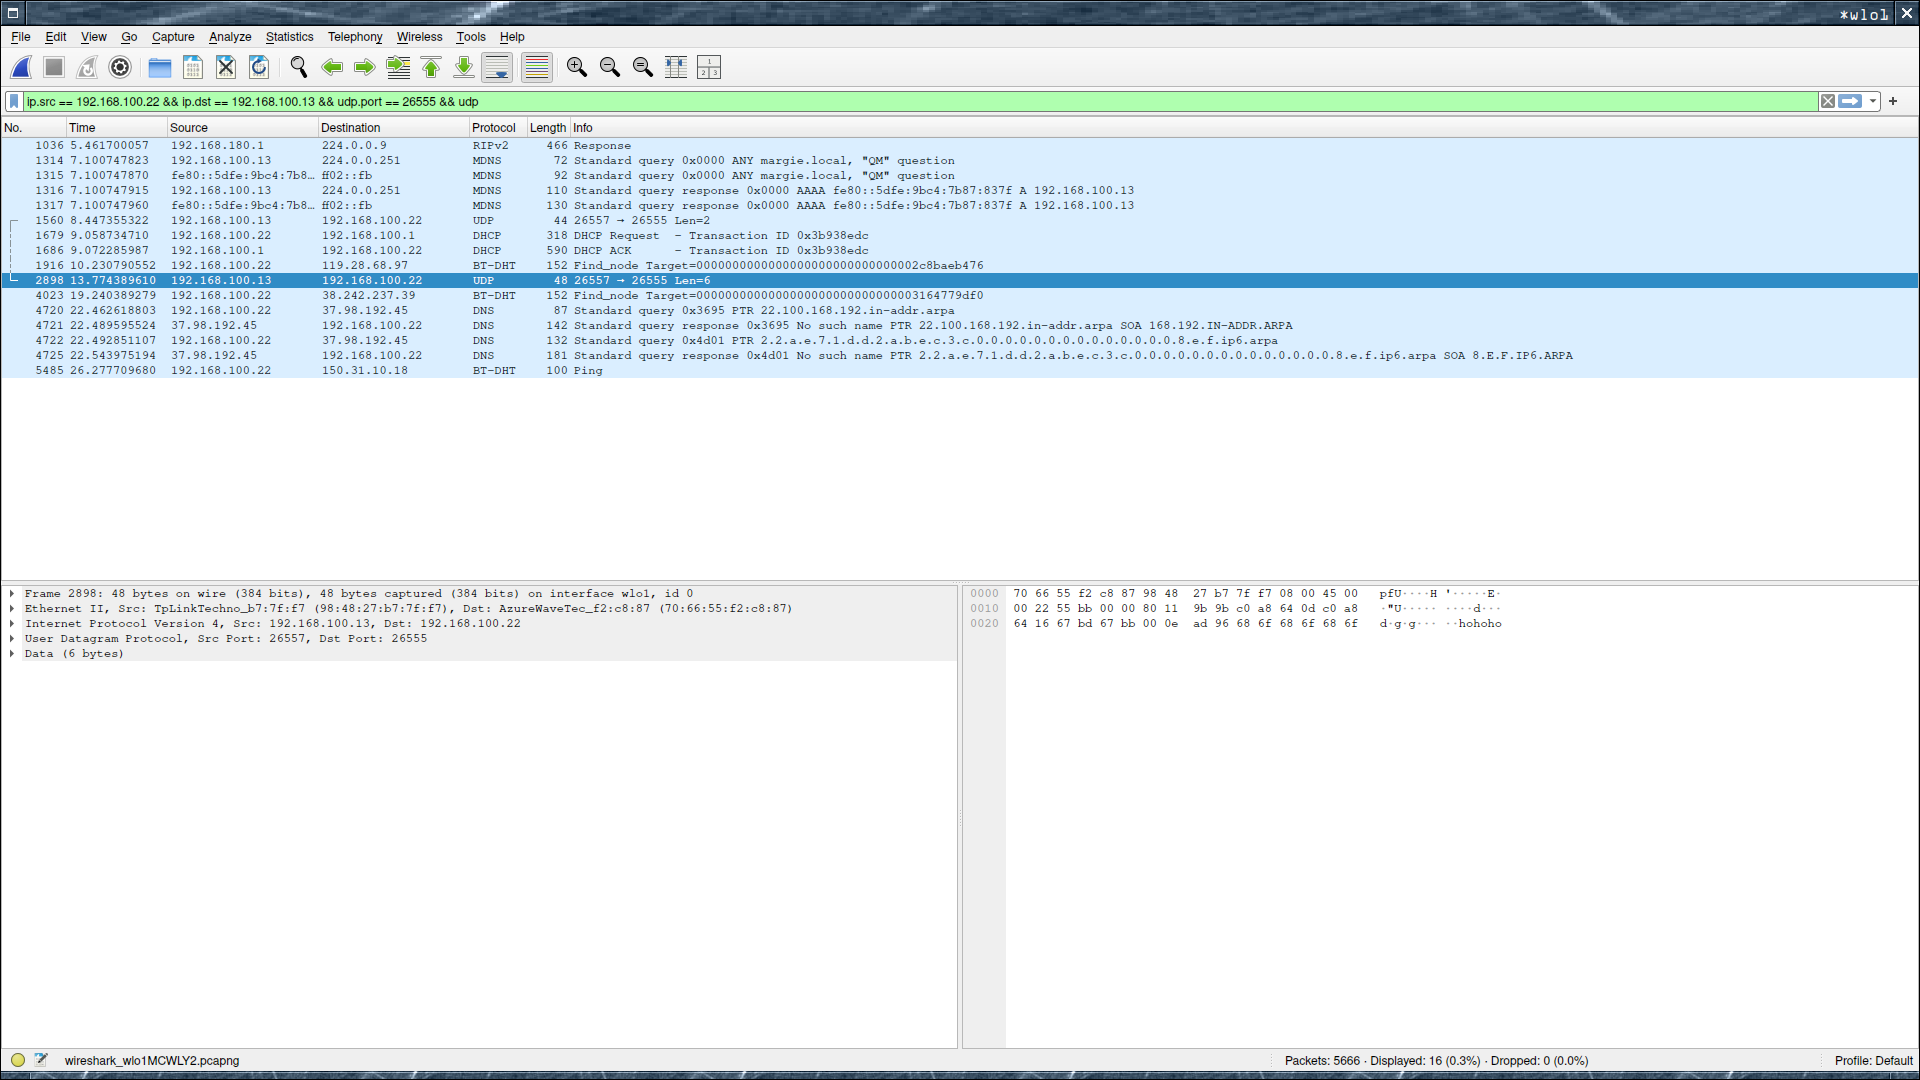
\includegraphics[scale=0.2]{text-simple-small.png}
    \caption{Καταγραφή μηνύματος μικρού μήκους στο Wireshark}\label{text-simple-n-small}
\end{figure}

Για την εικόνα~\ref{text-big} στείλαμε τον ίδιο τον πηγαίο κώδικα μέσω της εφαρμογής για να 
δοκιμάσουμε τη συμπεριφορά της σε πολύ μεγάλα κείμενα ($> 1024$ bytes). Βλέπουμε ότι το 
κείμενο χωρίζεται σε πολλά datagrams με μέγεθος payload $1024$ bytes μέχρι το τελευταίο
datagram στο οποίο στέλνεται ουσιαστικά ``ό,τι περίσσεψε''.

% change all filename underscores to dashes
\begin{figure}%
    \centering
    \begin{subfigure}{0.25\textwidth{}pt}
        \includegraphics[scale=0.3]{text\_big\_send.png}
    \end{subfigure}
    \begin{subfigure}
        \includegraphics[scale=0.3]{text\_big\_send.png}
    \end{subfigure}
    \begin{subfigure}
        \includegraphics[scale=0.3]{text\_big\_send.png}
    \end{subfigure}
    \caption{Παράδειγμα αποστολής πολύ μεγάλου κειμένου, χωρισμός σε πολλά μικρότερα πακέτα}\label{text-big}
\end{figure}
\section{VoIP}
\subsection{Receive}
\subsection{Send}
\subsection{Παράδειγμα VoIP μέσω Wireshark}
\section{Συμπεράσματα;}
\end{document}
